% Ist-Architektur.tex
\section{Ist-Architektur}

\begin{figure}[h]
  \caption{caption}
  \centering
  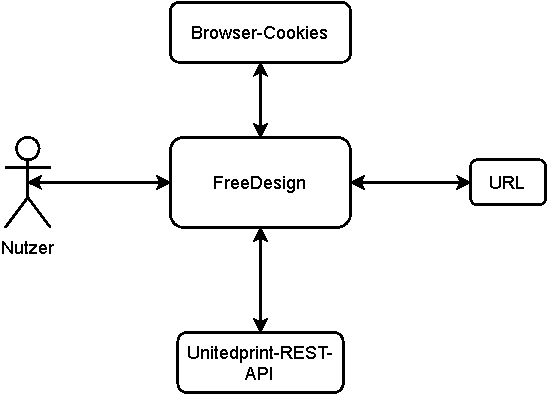
\includegraphics{diagrams/Freedesign_Interaktion.pdf}
\end{figure}
% Finden ein Dokumentationsform

% Vorgehensweise
% 1. Interviews

% Strategic Design
% 2. Ubiquitous Lang definieren


\subsection{Analyse Ist-Architektur}
Analyse der Ist-Architektur
\begin{itemize}
\item Hi­e­r­ar­chi­sie­rung
\item Paketstruktur und Zugriffe
\item Komponenten-Strukturierung
\item etc.
\end{itemize}

\subsection{Bewertung Ist-Architektur}
Kritische Bewertung der Ist-Architektur auf Schwächen.
\begin{itemize}
\item Einhaltung von SOLID
\item Design-Smells
\item Zyklen
\item etc.
\end{itemize}
